%!TEX root=../Benutzerhandbuch.tex
\chapter{Installation}
\section{Start der Installation}
Die Installation wird durch das ausf�hren der setup.exe gestartet. Danach �ffnet sich der Installer.
\begin{figure}[H]
\centering
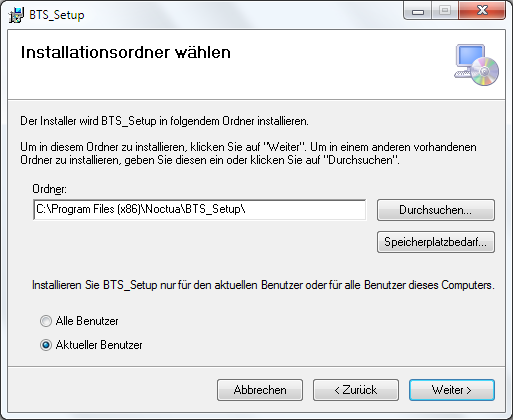
\includegraphics[width=1\textwidth]{images/btsinstall1.png}
\caption{Konfigurieren der Installtion}
\end{figure}
Nach der korrekten Konfiguration des Setups kann die Installtion gestartet werden.
\begin{figure}[H]
\centering
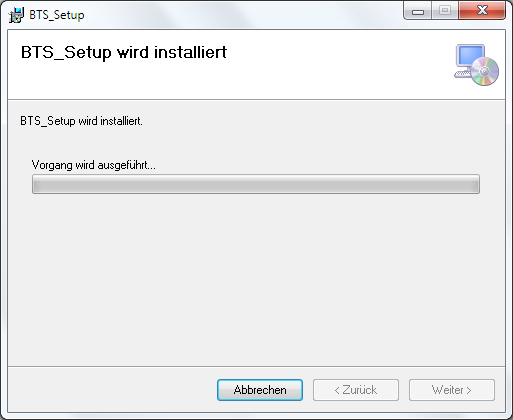
\includegraphics[width=1\textwidth]{images/btsinstall2.png}
\caption{Installationsvorgang}
\end{figure}
Nach diesem Vorgang ist die Backtesting-Software vollst�ndig installiert und ausf�hrbar.